\section{Thiết kế hệ thống}

\subsection{Tổng quan hệ thống}
Để đáp ứng yêu cầu xử lý thời gian thực, đồng bộ hóa luồng dữ liệu phức tạp từ cảm biến và tối ưu hóa tài nguyên phần cứng, hệ thống được thiết kế dựa trên kiến trúc \textbf{đa tác vụ} chạy trên nền tảng \textbf{Hệ điều hành thời gian thực FreeRTOS} nhúng trong vi điều khiển lõi kép \textbf{ESP32-S3 (Yolo UNO)}.

Toàn bộ các tác vụ xử lý bao gồm đọc dữ liệu cảm biến, hiển thị LCD, điều khiển LED/NeoPixel cảnh báo, thực thi mô hình trí tuệ nhân tạo biên (TinyML), chạy máy chủ Web Server cục bộ và đồng bộ dữ liệu đám mây (CoreIOT) được thiết kế chạy song song độc lập. Các tác vụ này tương tác và chia sẻ tài nguyên một cách an toàn thông qua các cơ chế đồng bộ hóa luồng của FreeRTOS như \textbf{Mutex} và \textbf{Semaphore}, giúp loại bỏ hoàn toàn các biến toàn cục không an toàn.

Sơ đồ kết nối phần cứng chi tiết của hệ thống được thể hiện trong Hình \ref{fig:sys_block_diagram}. 

\begin{figure}[H]
    \centering
    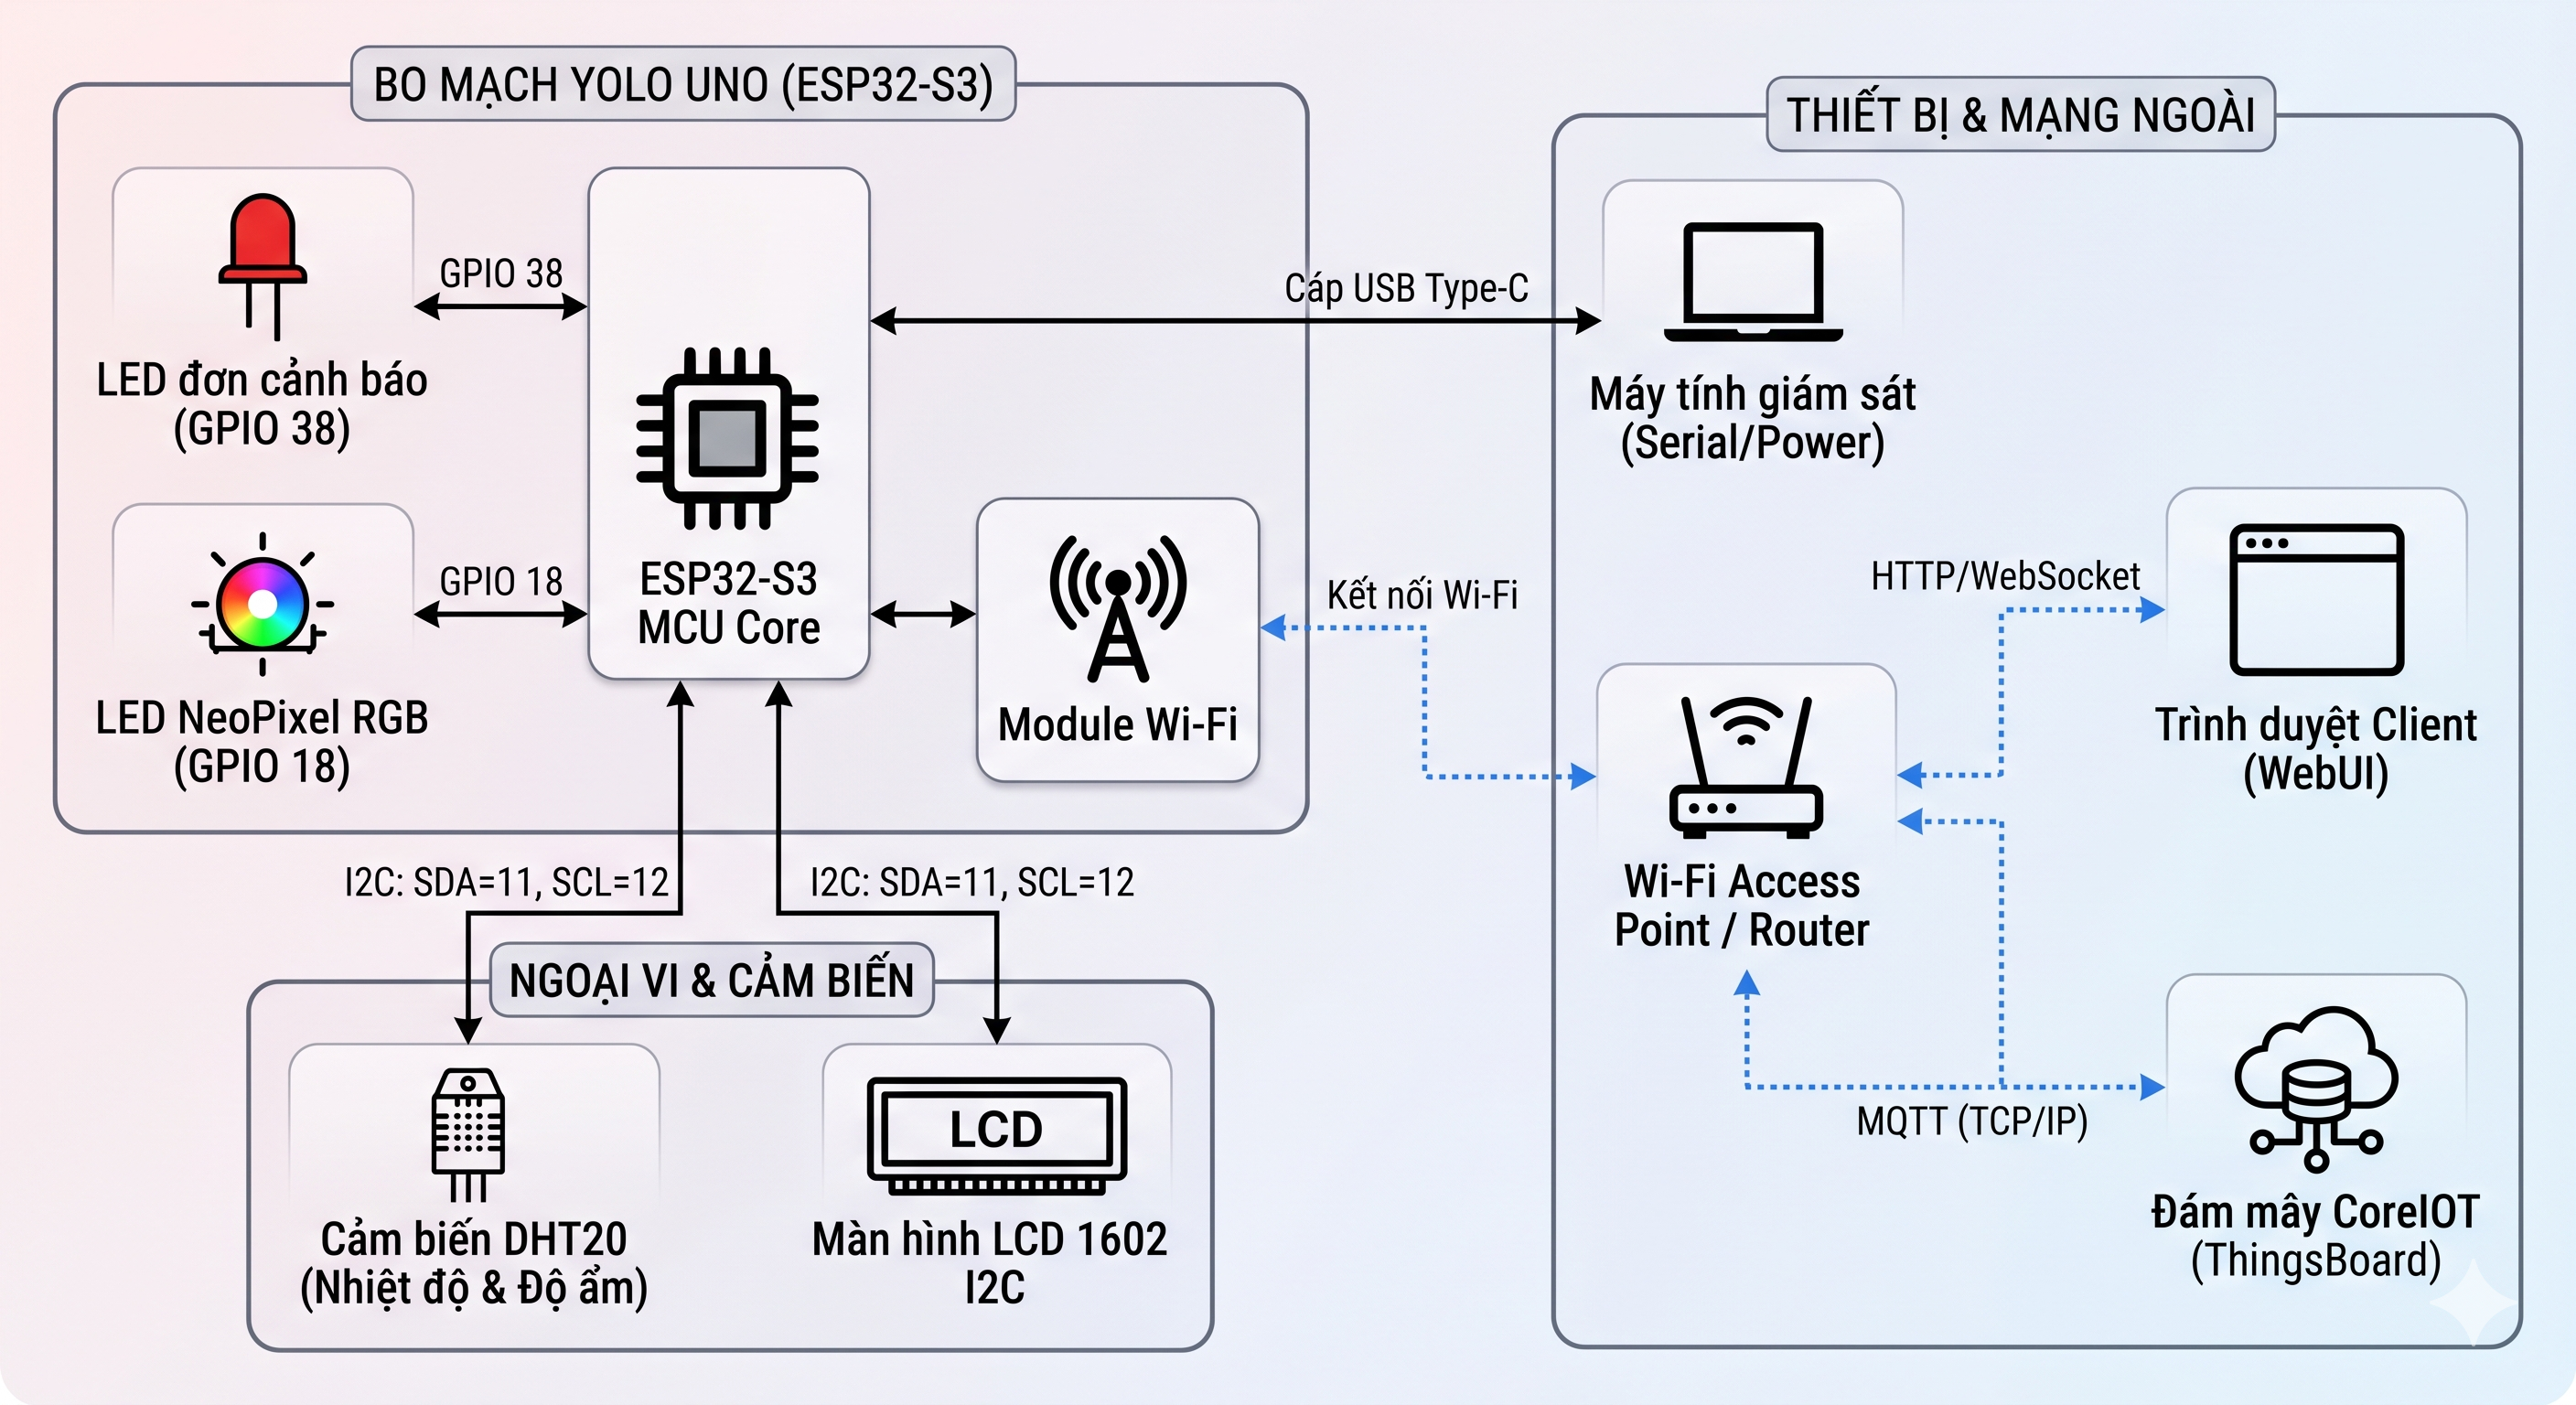
\includegraphics[width=0.8\textwidth]{SourceImage/sys_block_diagram.png}
    \caption{Sơ đồ khối tổng quan kết nối phần cứng hệ thống}
    \label{fig:sys_block_diagram}
\end{figure}

Qua sơ đồ này, vi điều khiển ESP32-S3 đóng vai trò là bộ xử lý trung tâm, thu thập dữ liệu từ cảm biến DHT20 qua giao thức I2C (sử dụng hai đường truyền tín hiệu SDA tại chân GPIO 11 và SCL tại chân GPIO 12) và chỉ thị trạng thái ra màn hình LCD 1602 (cũng kết nối chung bus I2C). Các cơ cấu hiển thị cảnh báo cục bộ khác gồm đèn LED đơn cảnh báo được điều khiển qua chân GPIO 38 và LED NeoPixel RGB qua chân GPIO 18. Thiết bị được cấp nguồn và giao tiếp gỡ lỗi với máy tính giám sát thông qua cáp USB Type-C. Đồng thời, module Wi-Fi tích hợp thiết lập liên kết không dây với Router trong mạng nội bộ để hỗ trợ giao tiếp WebSocket với các thiết bị khách và giao thức MQTT với máy chủ đám mây CoreIOT (ThingsBoard).

Kiến trúc đa tác vụ song song của hệ thống dưới sự quản lý của FreeRTOS được mô tả chi tiết trong Hình \ref{fig:arch_rtos}.

\begin{figure}[H]
    \centering
    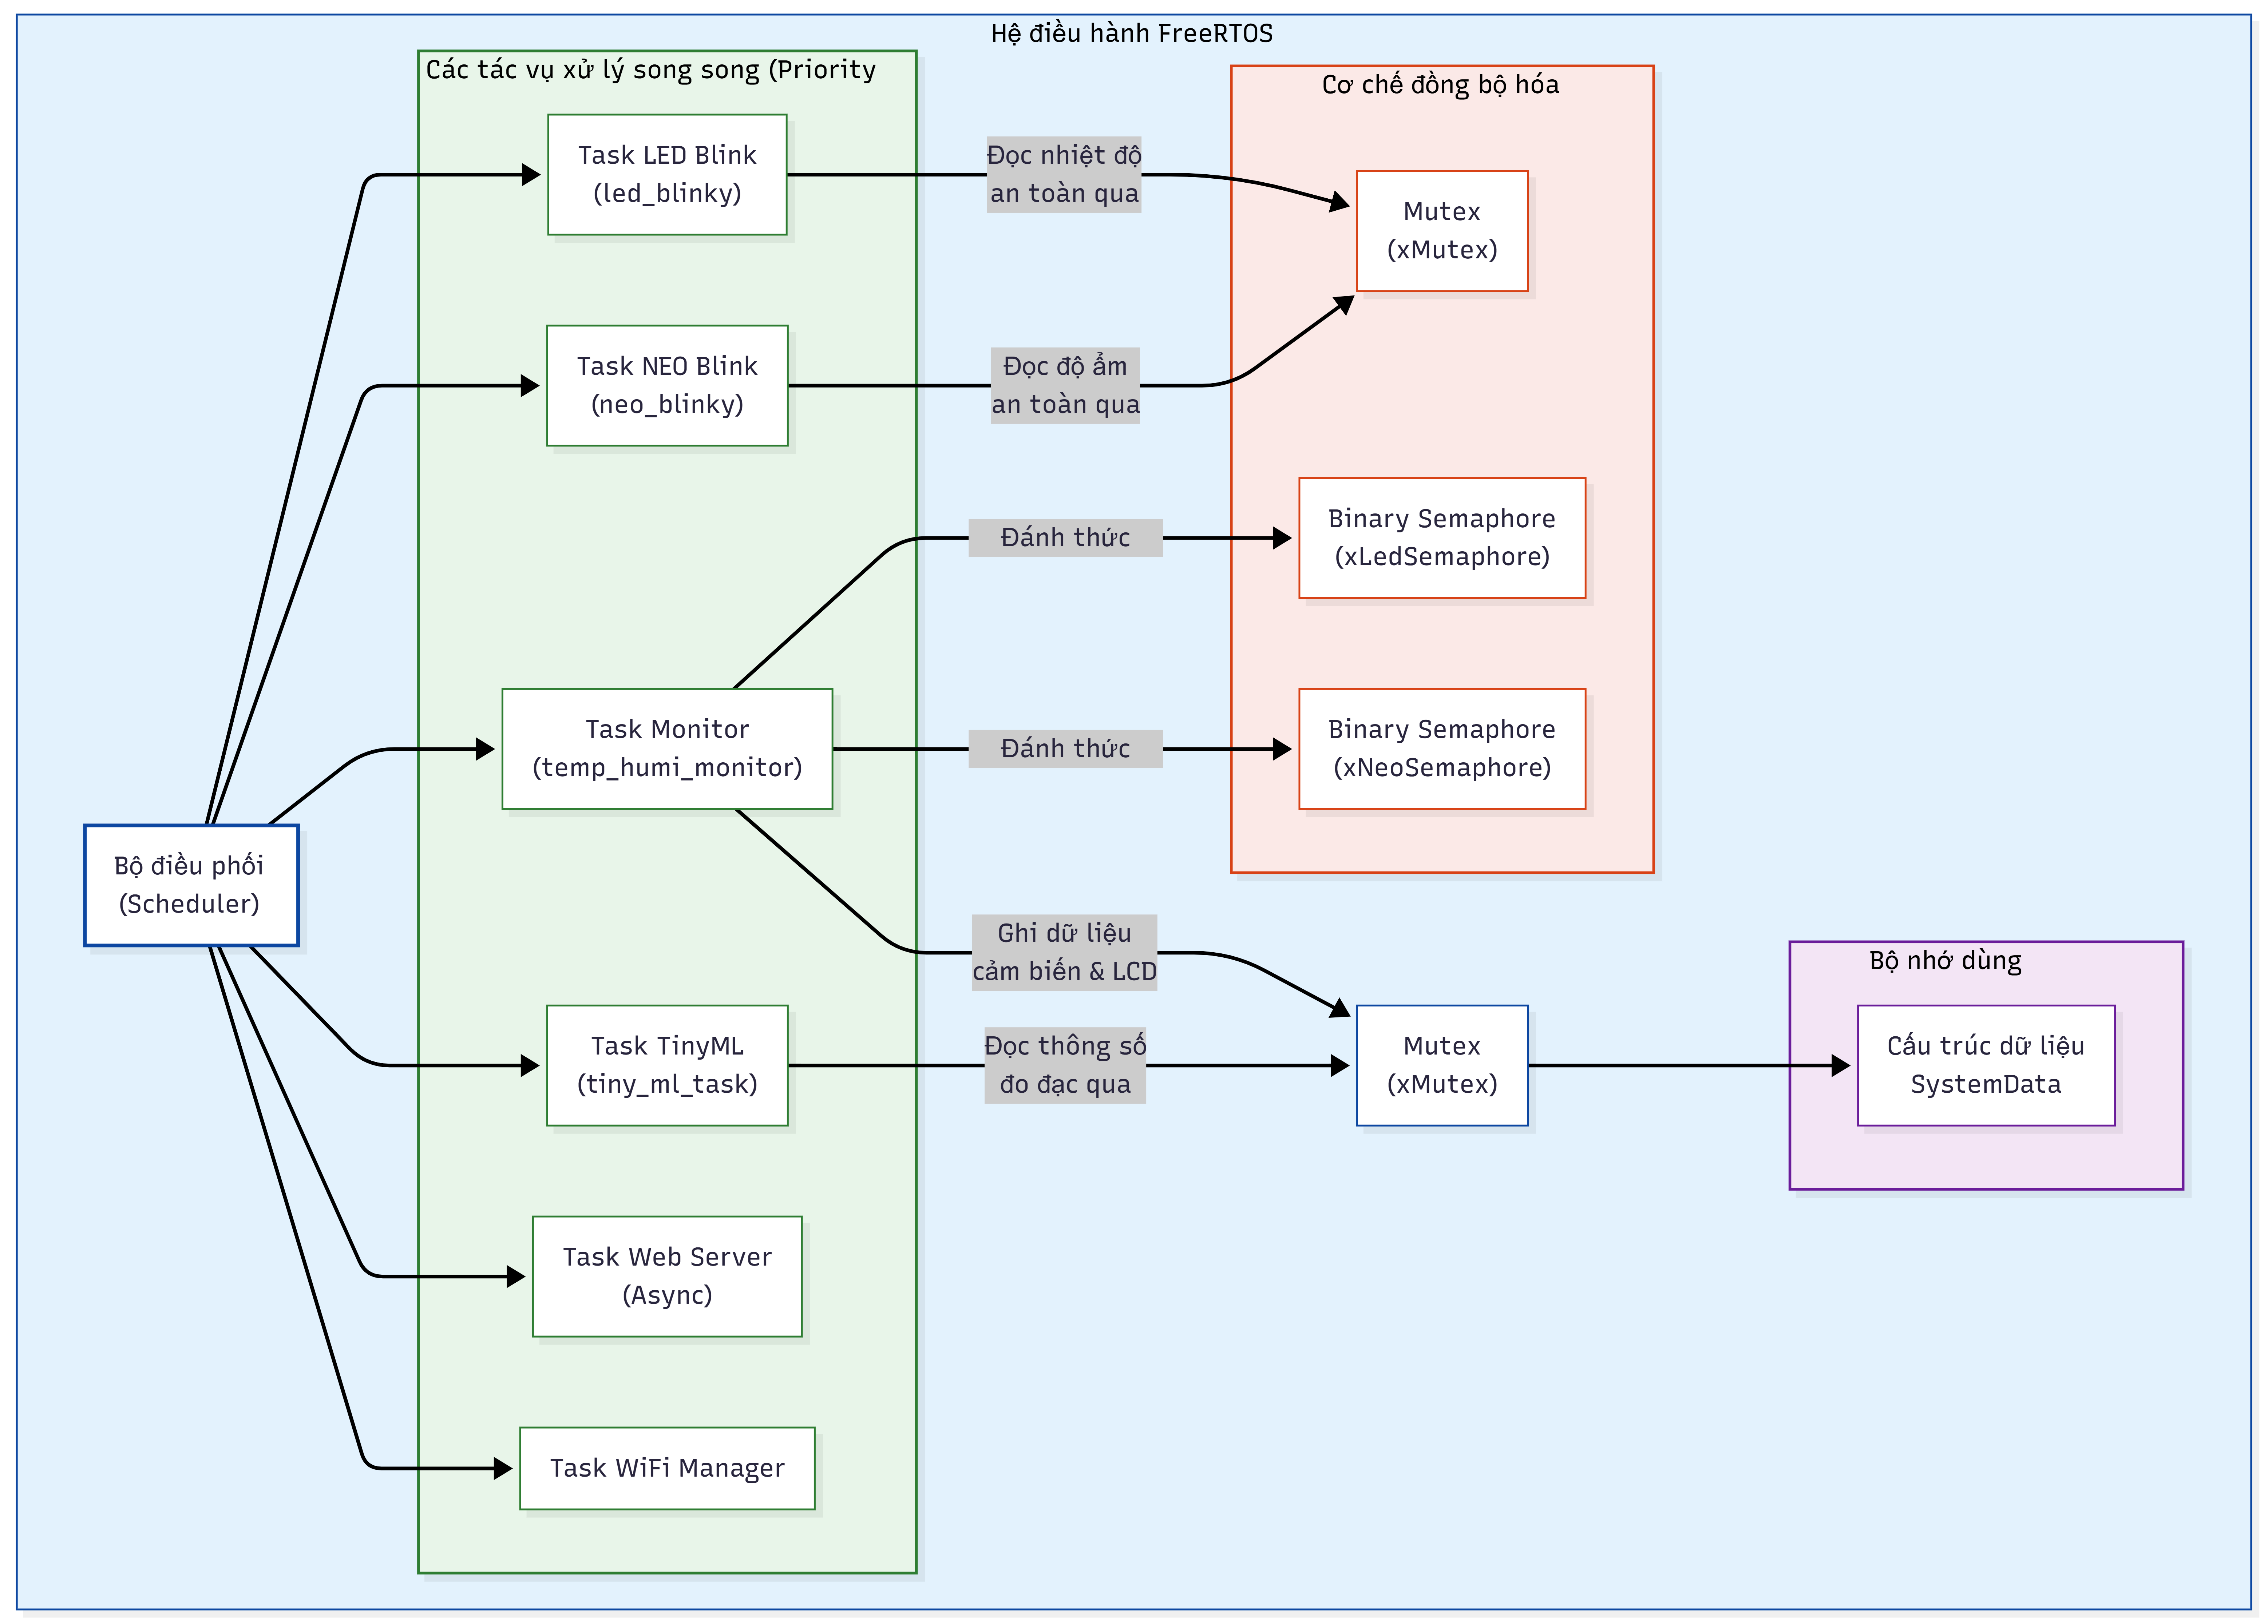
\includegraphics[width=0.8\textwidth]{SourceImage/arch_rtos.png}
    \caption{Kiến trúc đa tác vụ hoạt động song song dưới sự điều phối của FreeRTOS trên bo mạch Yolo UNO}
    \label{fig:arch_rtos}
\end{figure}

Kiến trúc này thể hiện việc hệ thống phân chia công việc thành 6 tác vụ (Tasks) chạy song song với độ ưu tiên bằng nhau (Priority 2): Task LED Blink, Task NEO Blink, Task Monitor, Task TinyML, Task Web Server và Task WiFi Manager. Các tác vụ này tương tác gián tiếp với nhau thông qua cấu trúc dữ liệu dùng chung \texttt{SystemData}. Để loại bỏ hiện tượng tranh chấp tài nguyên trên bus I2C và vùng nhớ dùng chung, hệ thống áp dụng cơ chế đồng bộ hóa thông qua Mutex (\texttt{xMutex}) bảo vệ. Ngoài ra, Task Monitor đóng vai trò là nguồn phát tín hiệu, định kỳ giải phóng các Semaphore nhị phân (\texttt{xLedSemaphore} và \texttt{xNeoSemaphore}) để đánh thức các tác vụ cảnh báo LED đơn và NeoPixel khi có dữ liệu cảm biến mới.

\subsection{Khối hiển thị LED, NeoPixel và LCD (Cảnh báo cục bộ)}
Khối chức năng hiển thị và cảnh báo cục bộ chịu trách nhiệm tương tác trực quan với người dùng tại chỗ. Để tránh xung đột tài nguyên và đồng bộ hóa các chu kỳ hiển thị theo chu kỳ đọc cảm biến, hệ thống thiết kế các tác vụ riêng biệt được đồng bộ hóa thời gian thực:
\begin{itemize}
    \item \textbf{Tác vụ điều khiển LED đơn (Task 1):} Tác vụ này duy trì Blocked State để tiết kiệm CPU và chỉ thức dậy khi nhận được tín hiệu giải phóng từ \textbf{Binary Semaphore} (\texttt{xLedSemaphore}) từ tác vụ đọc cảm biến. Tác vụ sẽ kiểm tra giá trị nhiệt độ hiện tại để điều khiển tần số nhấp nháy của LED theo 3 dải cảnh báo riêng biệt (an toàn, cảnh báo, khẩn cấp).
    \item \textbf{Tác vụ điều khiển LED NeoPixel (Task 2):} Tương tự như LED đơn, tác vụ điều khiển màu sắc của dải LED RGB NeoPixel được đồng bộ qua \textbf{Binary Semaphore} (\texttt{xNeoSemaphore}). Tác vụ ánh xạ mức độ ẩm nhận được thành 3 màu sắc đại diện (Đỏ - khô hạn, Xanh lá - lý tưởng, Xanh dương - ẩm ướt) mà không gây trễ giao diện.
    \item \textbf{Tác vụ hiển thị LCD I2C (Task 3):} Tác vụ này kiểm soát màn hình LCD 1602 giao tiếp qua I2C. Để ngăn ngừa hiện tượng tranh chấp đường truyền bus I2C (Race Condition) khi ghi thông số cảm biến, hệ thống sử dụng \textbf{Mutex} (\texttt{xMutex}) để độc chiếm tài nguyên bus I2C một cách an toàn. Màn hình tự động cập nhật nhiệt độ, độ ẩm thực tế và thay đổi linh hoạt giữa 3 trạng thái giao diện: ``NORMAL'', ``WARNING'', và ``CRITICAL''.
\end{itemize}

\begin{figure}[H]
    \centering
    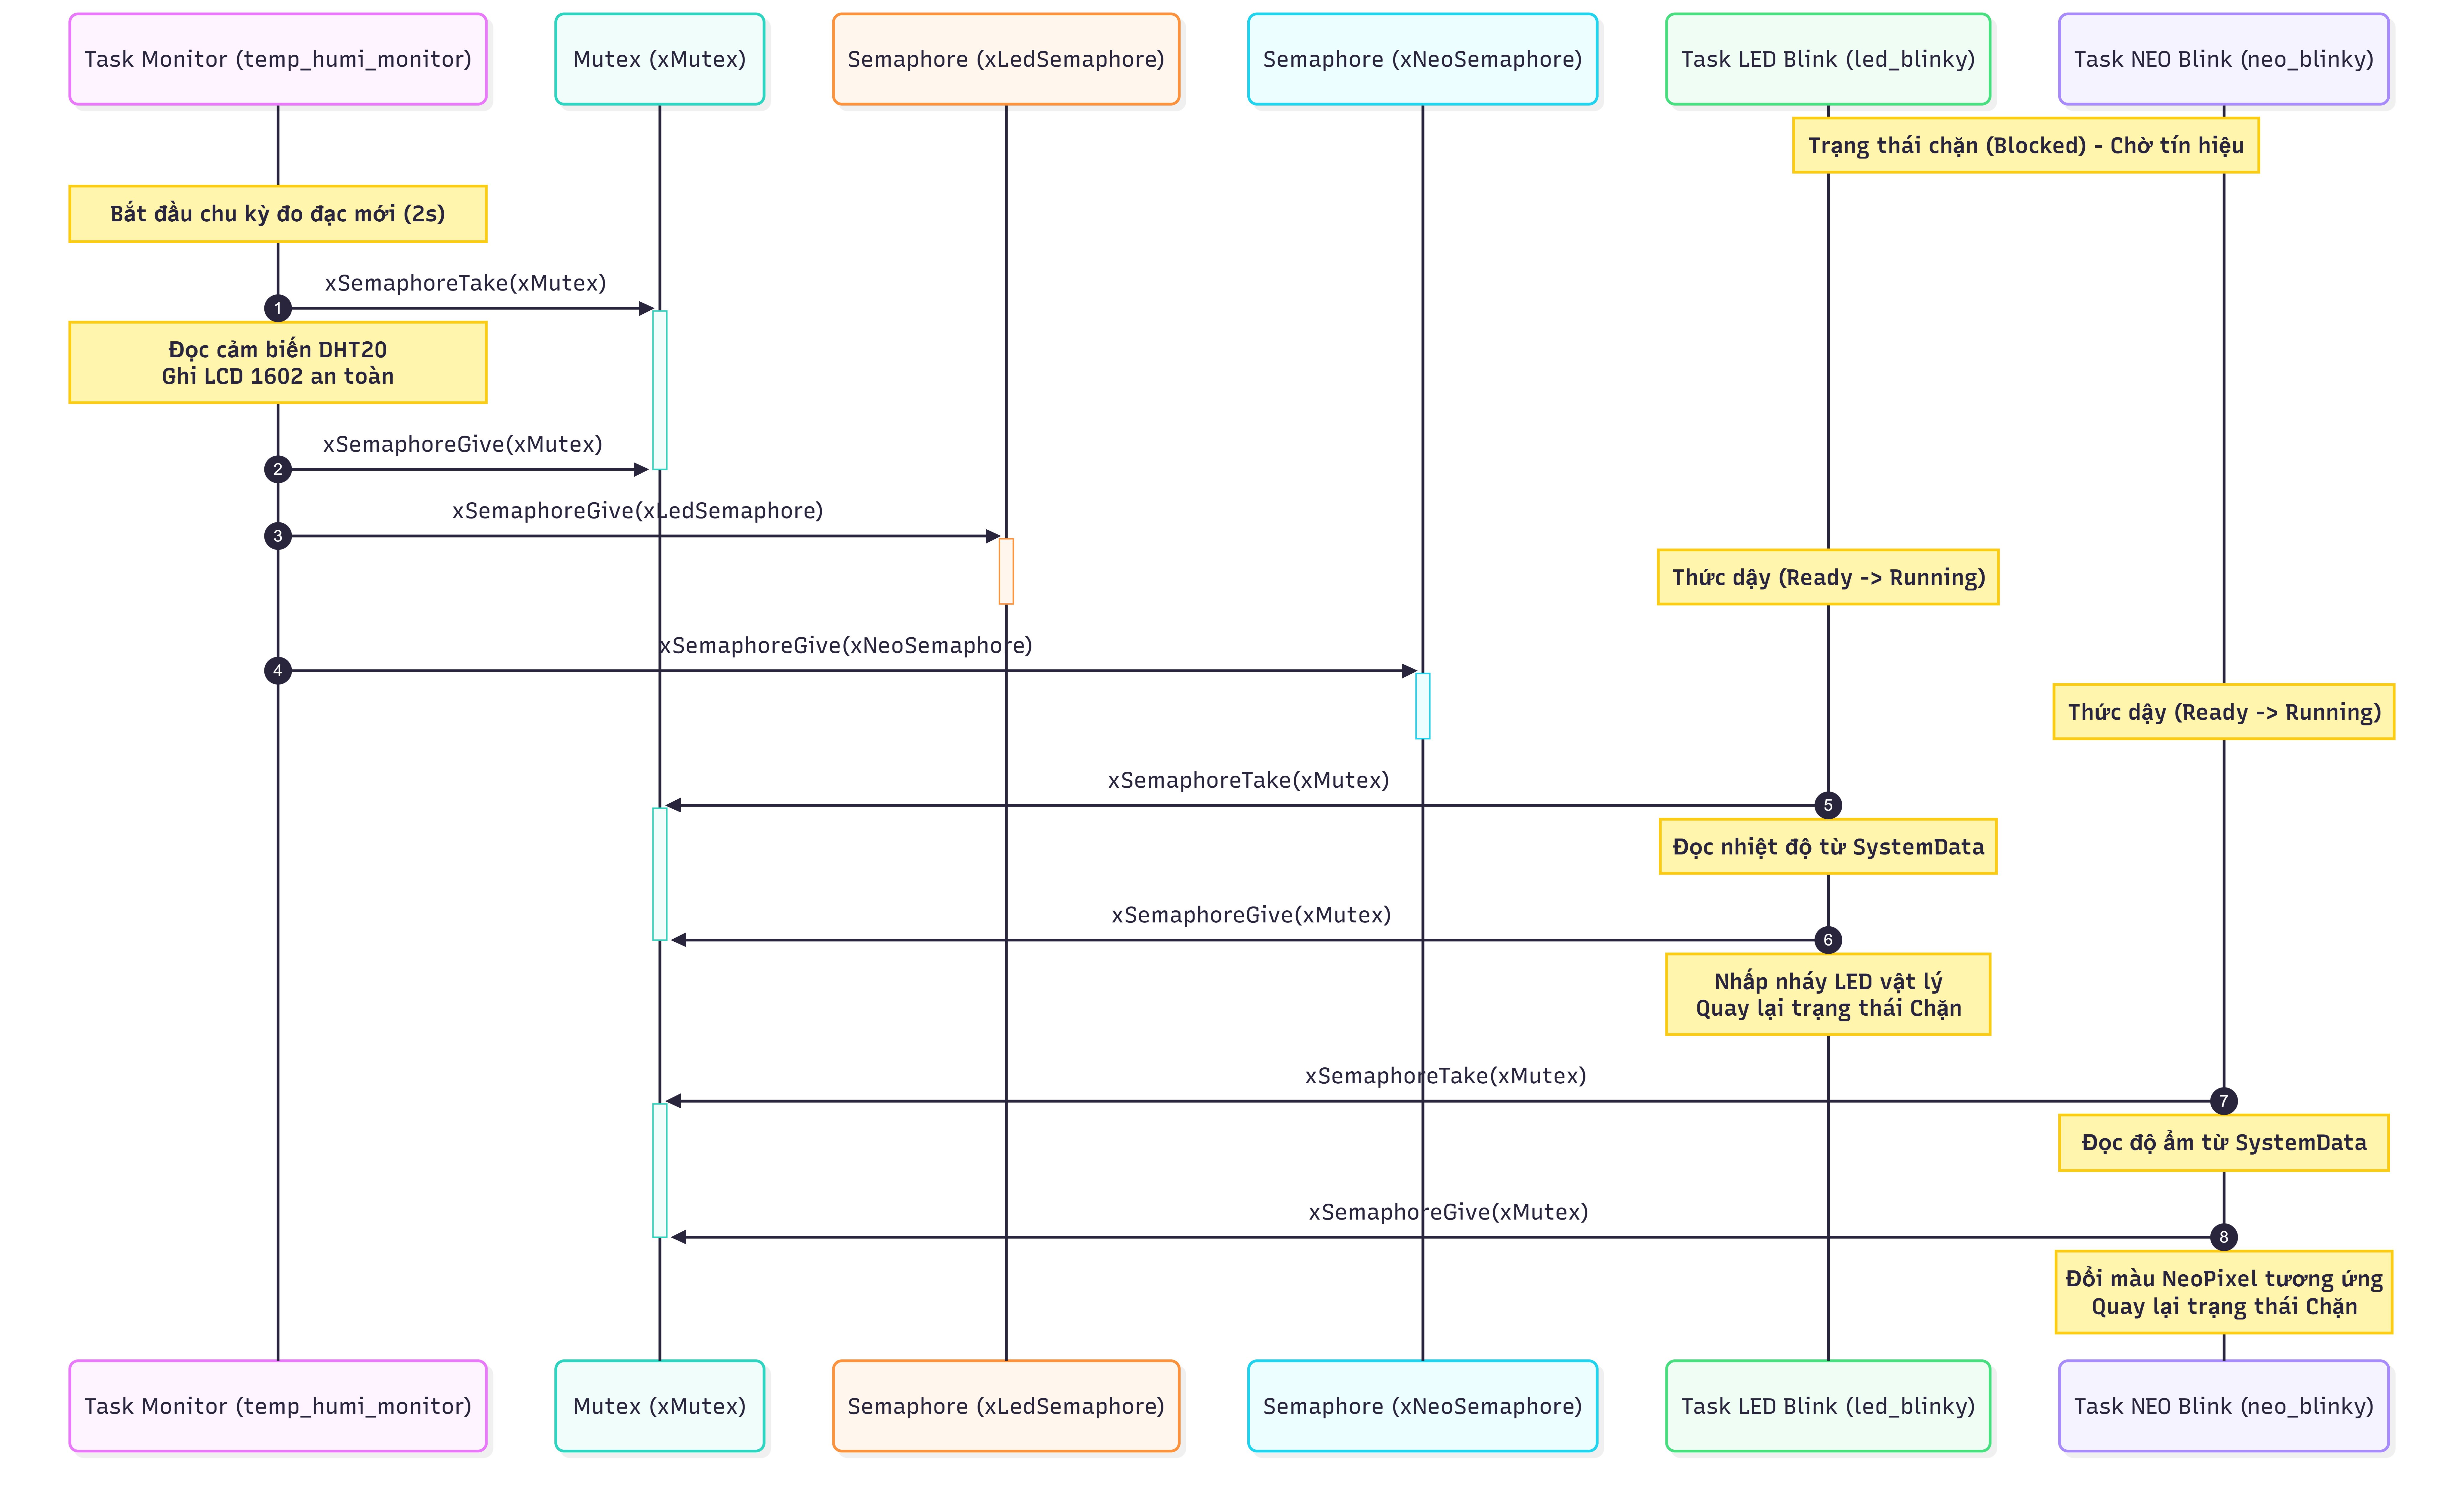
\includegraphics[width=0.8\textwidth]{SourceImage/sync_diagram.png}
    \caption{Cơ chế đồng bộ hóa đa tác vụ cảnh báo cục bộ qua Semaphore và Mutex}
    \label{fig:sync_diagram}
\end{figure}

Cơ chế đồng bộ hóa chi tiết giữa ba tác vụ hiển thị và cảnh báo cục bộ thông qua các Semaphore và Mutex được thể hiện trực quan trong Hình \ref{fig:sync_diagram}. Quy trình đồng bộ hóa bắt đầu khi Task Monitor khởi chạy chu kỳ đo đạc mới (mỗi 2 giây). Ban đầu, các Task LED Blink và Task NEO Blink ở trạng thái Chặn để nhường CPU. Task Monitor yêu cầu chiếm Mutex \texttt{xMutex} để độc quyền ghi dữ liệu từ cảm biến DHT20 lên màn hình LCD 1602 một cách an toàn, tránh xung đột bus I2C. Sau khi hoàn tất và trả lại Mutex, Task Monitor thực hiện gọi \texttt{xSemaphoreGive} cho hai Semaphore nhị phân \texttt{xLedSemaphore} và \texttt{xNeoSemaphore} để đánh thức các tác vụ phụ. Khi thức dậy, Task LED Blink và Task NEO Blink lần lượt chiếm Mutex \texttt{xMutex} trong khoảng thời gian rất ngắn để đọc giá trị nhiệt độ, độ ẩm an toàn từ cấu trúc dữ liệu chung, sau đó thực thi điều khiển nhấp nháy LED vật lý hoặc chuyển đổi màu sắc NeoPixel trước khi quay trở lại trạng thái chặn. Thiết kế này đảm bảo việc truy cập tài nguyên LCD không bị xung đột và tần số nhấp nháy/màu sắc của LED được cập nhật ngay lập tức khi có dữ liệu cảm biến mới.

\subsection{Khối Webserver + Điều khiển cục bộ (Task 4)}
Khối truyền thông điều khiển cục bộ cung cấp một máy chủ Web Server tích hợp trực tiếp trên chip ESP32-S3, cho phép người dùng giám sát và cấu hình thiết bị từ xa qua mạng nội bộ:
\begin{itemize}
    \item \textbf{Máy chủ Web Asynchronous:} Sử dụng thư viện máy chủ không đồng bộ (\texttt{ESPAsyncWebServer}), giúp phản hồi nhanh các yêu cầu HTTP mà không gây nghẽn các tác vụ RTOS khác. Toàn bộ các tệp tin giao diện WebUI được lưu trữ trực tiếp trong bộ nhớ Flash của chip dưới dạng hệ thống tệp tin tĩnh.
    \item \textbf{Giao tiếp WebSocket:} Thay vì sử dụng HTTP REST API truyền thống, hệ thống thiết kế kênh truyền thông song công \textbf{WebSocket} (\texttt{AsyncWebSocket}) để truyền dữ liệu cảm biến dạng JSON theo thời gian thực tới giao diện người dùng và tiếp nhận tức thời lệnh điều khiển cơ cấu chấp hành (bật/tắt các cổng GPIO liên kết với LED/Relay).
\end{itemize}

\begin{figure}[H]
    \centering
    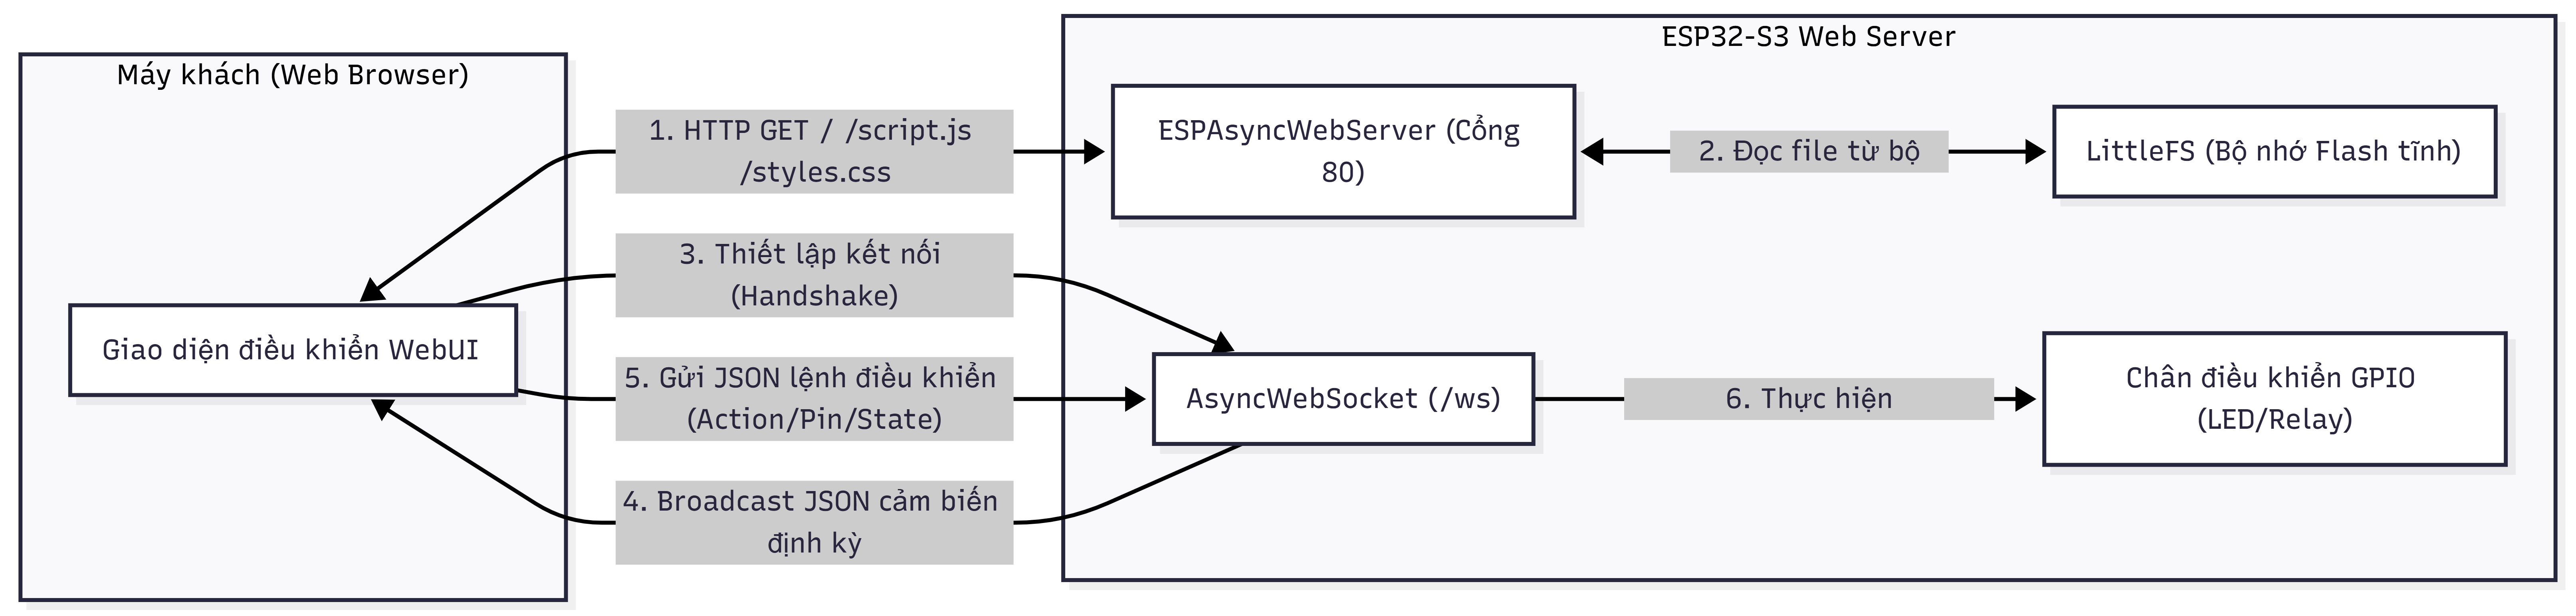
\includegraphics[width=0.8\textwidth]{SourceImage/web_communication_diagram.png}
    \caption{Sơ đồ giao tiếp truyền thông cục bộ qua WebServer và WebSocket}
    \label{fig:web_communication_diagram}
\end{figure}

Quy trình truyền nhận dữ liệu thời gian thực và lệnh điều khiển thiết bị thông qua giao thức WebSocket kết hợp máy chủ Web không đồng bộ được minh họa trong Hình \ref{fig:web_communication_diagram}. Ở giai đoạn khởi động, khi Web Client truy cập địa chỉ thiết bị, máy chủ Web Asynchronous (\texttt{ESPAsyncWebServer}) sẽ tiếp nhận yêu cầu HTTP GET và đọc các tệp tĩnh gồm \texttt{index.html}, \texttt{script.js}, \texttt{styles.css} từ bộ nhớ Flash tĩnh định dạng hệ thống tệp tin LittleFS để trả về cho trình duyệt. Sau khi tải xong trang web, trình duyệt sẽ chủ động khởi tạo một kết nối WebSocket Handshake thông qua endpoint \texttt{/ws} để thiết lập kênh truyền song công liên tục. Thông qua kênh này, Server định kỳ đóng gói dữ liệu cảm biến thành chuỗi JSON và gửi broadcast tới mọi client đang kết nối để cập nhật đồ thị giao diện thời gian thực. Ngược lại, khi người dùng tương tác trên WebUI, Web Client sẽ gửi gói tin JSON chứa các lệnh điều khiển (\texttt{action}, \texttt{pin}, \texttt{state}) lên server để thực hiện hàm \texttt{digitalWrite} tác động trực tiếp vào các chân GPIO ngoại vi (LED, Relay). WebSocket giúp duy trì kết nối song công liên tục, giảm thiểu băng thông và tăng tốc độ phản hồi lệnh điều khiển từ người dùng.

\subsection{Khối CoreIOT + Kết nối mạng STA (Task 6)}
Khối tương tác đám mây diện rộng đảm nhận việc đẩy dữ liệu lên máy chủ từ xa phục vụ giám sát tập trung:
\begin{itemize}
    \item \textbf{Cơ chế kết nối WiFi STA:} Khi có cấu hình mạng hợp lệ, thiết bị kích hoạt Wi-Fi ở chế độ STA để liên kết vào mạng bộ định tuyến có kết nối Internet.
    \item \textbf{Đẩy dữ liệu Cloud qua MQTT:} Tác vụ định kỳ đóng gói giá trị nhiệt độ và độ ẩm vào gói tin JSON, sau đó sử dụng thư viện ThingsBoard MQTT kết hợp với Device Token để xuất bản dữ liệu viễn trắc lên máy chủ đám mây CoreIOT~\cite{coreiot}.
\end{itemize}

\subsection{Khối TinyML (Task 5)}
Khối trí tuệ nhân tạo nhúng chạy trực tiếp thuật toán học máy tại biên để phát hiện bất thường môi trường:
\begin{itemize}
    \item \textbf{Mô hình TensorFlow Lite Micro:} Mô hình FFN được huấn luyện từ trước và nhúng trực tiếp dưới dạng mảng hằng số C. Dữ liệu nhiệt độ và độ ẩm dạng \texttt{float32} được nạp trực tiếp làm đầu vào cho mô hình suy luận.
    \item \textbf{Bộ nhớ Tensor Arena tĩnh:} Để tránh lỗi phân mảnh bộ nhớ động trên hệ thống thời gian thực, bộ thông dịch TensorFlow Lite Micro được cấp phát một vùng nhớ tĩnh 8~kB cố định trên RAM.
    \item \textbf{Tự đánh giá khi khởi động (Startup Test):} Nhằm đo lường độ chính xác của mô hình ngay trên phần cứng, hệ thống tích hợp tập dữ liệu kiểm thử gồm 50 mẫu tĩnh. Khi khởi động, tác vụ TinyML sẽ chạy suy luận trên toàn bộ tập mẫu này và tính toán các chỉ số chất lượng gồm Accuracy, Precision, Recall và xuất ra cổng Serial.
\end{itemize}

\begin{figure}[H]
    \centering
    \includegraphics[width=0.6\textwidth]{SourceImage/tinyML_pipeline_diagram.png}
    \caption{Quy trình suy luận của mô hình TinyML trên thiết bị nhúng}
    \label{fig:tinyml_pipeline_diagram}
\end{figure}

Quy trình suy luận biên của mô hình TinyML được mô tả trong Hình \ref{fig:tinyml_pipeline_diagram}. Dữ liệu thô thu thập từ cảm biến DHT20 sẽ được ép kiểu dữ liệu về dạng số thực \texttt{float32} trước khi nạp vào vùng nhớ Tensor đầu vào. Bộ thông dịch TensorFlow Lite Micro đóng vai trò trung tâm xử lý, sử dụng mô hình mạng nơ-ron đã được nhúng tĩnh dưới dạng mảng byte (\texttt{model\_data.h}) và vùng nhớ đệm Arena tĩnh có kích thước cố định \textbf{8~kB} trên RAM để tiến hành thực thi hàm \texttt{interpreter->Invoke()}. Sau khi tính toán lan truyền thẳng qua các lớp mạng nơ-ron, kết quả suy luận được lưu vào Tensor đầu ra dưới dạng một Điểm bất thường. Hệ thống sẽ so sánh điểm số này với một ngưỡng cài đặt trước (0.5): nếu điểm số vượt ngưỡng, thiết bị xác định trạng thái môi trường là Bất thường, ngược lại là Bình thường. Kết quả này sẽ được xuất trực tiếp ra cổng Serial và cập nhật lên màn hình LCD cục bộ.

\subsection{Khối quản lý cấu hình và Định danh thiết bị (LittleFS)}
Hệ thống được thiết kế để hoạt động động và linh hoạt mà không cần nạp lại chương trình khi thay đổi môi trường:
\begin{itemize}
    \item \textbf{Lưu trữ cấu hình động bằng LittleFS:} Toàn bộ thông tin kết nối Wi-Fi (SSID, Password) và thông tin cấu hình đám mây CoreIOT (Server, Token, Port) được lưu trữ dưới dạng tệp tin JSON `/info.dat` trong phân vùng LittleFS trên bộ nhớ Flash. Khi khởi động, hệ thống đọc tệp tin này; nếu chưa cấu hình, thiết bị sẽ tự động khởi tạo Access Point phát Wi-Fi để người dùng nhập thông tin. Sau khi nhận được thông tin cấu hình từ WebUI, thiết bị lưu lại và tự khởi động lại vào chế độ STA kết nối Internet.
    \item \textbf{Định danh bằng MAC Address:} Hệ thống sử dụng địa chỉ vật lý MAC Address mặc định của phần cứng chip Wi-Fi để tạo thuộc tính định danh thiết bị độc bản gửi lên CoreIOT, giúp quản lý và định danh chính xác thiết bị trên máy chủ.
\end{itemize}

\begin{figure}[H]
    \centering
    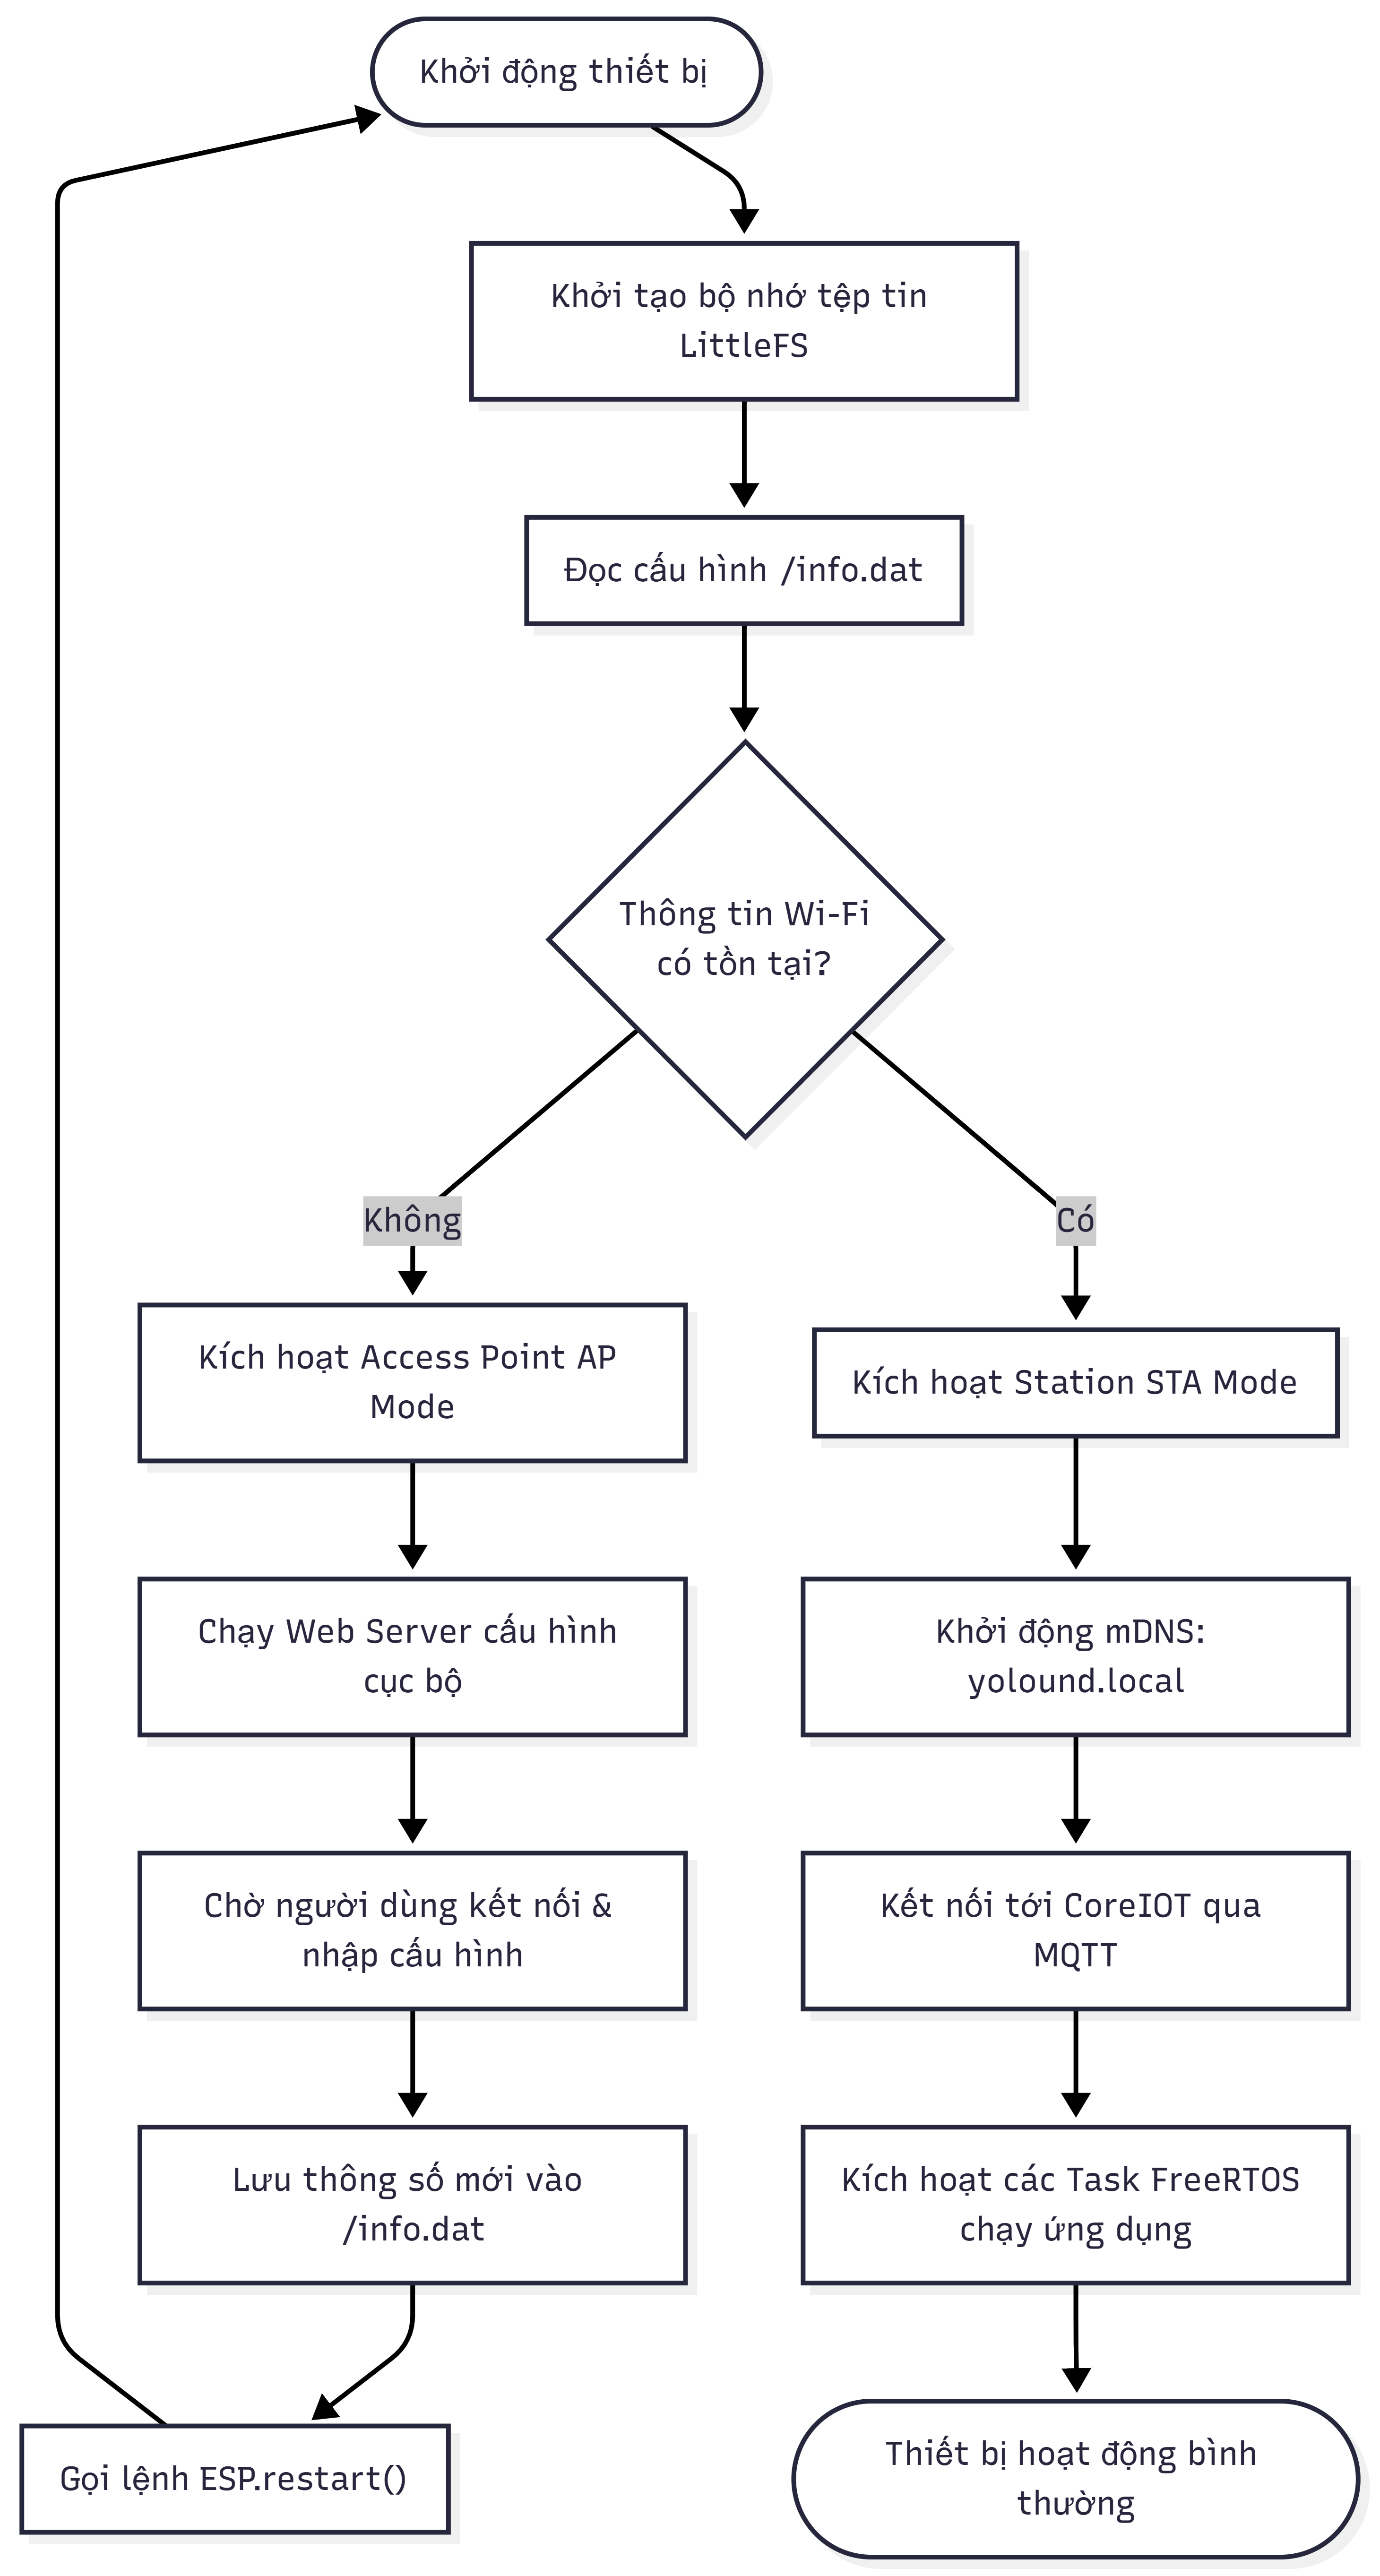
\includegraphics[width=0.6\textwidth]{SourceImage/config_flowchart.png}
    \caption{Lưu đồ thuật toán quản lý cấu hình động bằng LittleFS}
    \label{fig:config_flowchart}
\end{figure}

Lưu đồ thuật toán quản lý cấu hình và khởi động động của hệ thống sử dụng hệ thống tệp tin LittleFS được mô tả trong Hình \ref{fig:config_flowchart}. Ngay khi thiết bị được khởi động, hệ thống tiến hành khởi tạo phân vùng tệp tin LittleFS và tìm đọc tệp dữ liệu cấu hình cục bộ \texttt{/info.dat}. Tiếp theo, một khối điều kiện kiểm tra sự tồn tại của thông tin kết nối Wi-Fi:
\begin{itemize}
    \item Nếu thông tin chưa tồn tại (như khi vận hành lần đầu tiên), thiết bị sẽ tự động kích hoạt chế độ Access Point, phát mạng Wi-Fi cấu hình và khởi chạy máy chủ Web cục bộ. Thiết bị duy trì trạng thái chờ người dùng kết nối vào mạng để nhập thông số cấu hình mạng mới thông qua trang WebUI. Sau khi nhận được thông tin, hệ thống ghi đè cấu hình vào \texttt{/info.dat} và gọi lệnh restart phần cứng để bắt đầu chu kỳ khởi chạy mới.
    \item Nếu thông tin Wi-Fi đã tồn tại, thiết bị lập tức kích hoạt chế độ Station kết nối trực tiếp vào mạng nội bộ, khởi tạo dịch vụ tên miền mDNS \texttt{yolound.local}, kết nối MQTT tới máy chủ CoreIOT và kích hoạt các tác vụ RTOS để chuyển sang chế độ hoạt động bình thường.
\end{itemize}
Cơ chế này giúp thiết bị linh hoạt tự động chuyển đổi giữa chế độ cấu hình (AP Mode) và chế độ hoạt động bình thường (STA Mode).